\documentclass[letterpaper]{article}

\usepackage{natbib,alifeconf,amsmath,amsfonts}  %% The order is important


% *****************
%  Requirements:
% *****************
%
% - All pages sized consistently at 8.5 x 11 inches (US letter size).
% - PDF length <= 8 pages for full papers, <=2 pages for extended
%    abstracts (not including citations).
% - Abstract length <= 250 words.
% - No visible crop marks.
% - Images at no greater than 300 dpi, scaled at 100%.
% - Embedded open type fonts only.
% - All layers flattened.
% - No attachments.
% - All desired links active in the files.

% Note that the PDF file must not exceed 5 MB if it is to be indexed
% by Google Scholar. Additional information about Google Scholar
% can be found here:
% http://www.google.com/intl/en/scholar/inclusion.html.


% If your system does not generate letter format documents by default,
% you can use the following workflow:
% latex example
% bibtex example
% latex example ; latex example
% dvips -o example.ps -t letterSize example.dvi
% ps2pdf example.ps example.pdf


% For pdflatex users:
% The alifeconf style file loads the "graphicx" package, and
% this may lead some users of pdflatex to experience problems.
% These can be fixed by editing the alifeconf.sty file to specify:
% \usepackage[pdftex]{graphicx}
%   instead of
% \usepackage{graphicx}.
% The PDF output generated by pdflatex should match the required
% specifications and obviously the dvips and ps2pdf steps become
% unnecessary.


% Note:  Some laser printers have a serious problem printing TeX
% output. The use of ps type I fonts should avoid this problem.


\title{ALIFE2022 template}



\title{Inferring Dynamic Parameter Relations from Experimental Probability Distributions}
\author{Anonymous Author$^{1}$, Anonymous Author2$^{1,2}$ \\
\mbox{}\\
$^1$California Institute of Technology, Pasadena, CA 91125 \\
$^2$California State University, Northridge, CA 91330 \\
anon@ymous.com} % email of corresponding author


% For several authors from the same institution use the same number to
% refer to one address.
%
% If the names do not fit well on one line use
%         Author 1, Author 2 ... \\ {\Large\bf Author n} ...\\ ...
%
% If the title and author information do not fit in the area
% allocated, place \setlength\titlebox{<new height>} after the
% \documentclass line where <new height> is 2.25in



\begin{document}
\maketitle

\begin{abstract}
% Abstract length should not exceed 250 words
    We present a novel method for relating experimental probability
    distributions of multistable systems to the parameters of a
    multistable model. We demonstrate that when such probability 
    distributions are fixed this implies that there is a fixed
    set of relations among the model parameters. Such relations 
    can help make predictions of parameters that aren't measured
    from ones that are. We apply this method
    to the canonical example of a bistable dynamical system: the cubic
    system.
    As well as to two theoretical models one of planerian regeneration
    and one of infant prehension learning.
\end{abstract}

\section{Introduction}
Biological systems are characterized by their robust stability under
a wide range of conditions. This is in part achieved by the ability
of such systems to take on different stable states
depending on contextual factors. One set of mechanisms that allows for such 
behavior is the presence of multiple long term stable states. Multistability
appears in a vast range of biological process ranging from microscale
genetic networks to macroscale population interactions. Across many levels 
of time and space biological systems seem to be able to adapt to new contexts
by maintaining multiple dominant stable modes.

Multistability has also
emerged as a useful tool in a explaining a large range of experimental phenomena.
Unlike theoretical models however, in the experimental context stochasticity
is unavoidable. As a result a common empirical practice is to sample what 
would be in the model, many possible trajectories of the system until they
reach equilibrium. 
Such sampling leads to a distribution of the stable states expressed as 
probabilities. This allows the experimenter to characterize the attractor
landscape and identify the range of possible equilibria.

Developmental dynamics are a particularly interesting case of multistability. 
Developing systems whether behavioral or morphological demonstrate multistability 
that is not only context decedent but expresses deep regularity in the timing of 
state transitions. In the case of behavior this can be observed in the existence
of critical periods or the milestones like progression developmental stages. 
In the case of morphological development we see this in the stage structure of
embryogenesis. A mechanistic understanding of how such regularity emerges is 
still in it's infancy.

In the context of the probabilistic approach used to experimentally 
study multistability, this regularity manifests as an observable oddity.
The probability distributions of developing systems ending up in a given
state is uncharacteristically consistent across different individuals 
in what would seem to be different conditions. The intuitive assumption
would be that each system would show a unique probability distribution
dependent upon individual factors. Instead, we observe that the probability
distributions are consistently species specific rather than individual specific.

Two examples of this phenomenon are the regeneration of the planerian flatworm
and the learning of reach-to-grasp in infants. In the case of planerian
theoretical models reveal how under certain environmental conditions 
planerian can develop into two possible configurations. In a natural context
the planerian when cut in two will regrow. The tail will regrow a head and the
head will grow a tail. However, experimental data from the Levin lab shows that
if the local electrical potential in the environment changes it is possible for 
a worm head to grow another head. Even, stranger is that if the potential
is altered only slightly, cryptic worms will emerge. Cryptic worms when cut 
may grow another head or a tail. In the case of the tail the child worm is 
also cryptic, even if returned to a normally polarized environment. The oddity
is that as long as the worm is cryptic the head-tail growth probability is $70\%$
regardless of the degree of polarization. This fixed probability is unexpected 
based on the basic theoretical assumptions one would make based on models of the
system.

Similarly, infant
prehension can be modeled as bistable: reach without grasp as one state
and reach with grasp as another, the system expresses both possibilities in the right
environmental context. Although an unexpected experimental finding is that in
both cases: the probability distributions across surprisingly large changes
to the relevant context remains relatively static. Infants maintain an extended 
period in which grasping starts to occur at a fixed probability. This is not a gradual
increase but rather a phase transition where for an extended period of time the probabilty
of reaching with and without grasping stays the same.
From a theoretical standpoint this seems 
counter-intuitive since changes over time and across infants would be expected 
to shift the basins of attraction and hence change the resultant probability 
distribution. Instead we see a period of relatively static probability.

Although, the source of this phenomena may be system specific and rely on deep
biological principles it serves as a fascinating example where the theoretical 
tools of dynamical systems could serve as a means of making experimental predictions.
In this work we propose a method to exploit such multistable regularity. We consider
theoretical models for both of these phenomena and identify how fixed 
probabilities provide a set of constraints on the relationship between model
parameters. This allows us to make predictions as to what various parameter 
values should be. We start by demonstrating the method in a simplified model
of bistability  then extend it to models of both flatworm regeneration and
prehension development.

\section{The Method}
In the following sections we first introduce our method by motivating
and applying it to a toy model which is a popular mathematical model
of bistability. Once we work through the method in this simplified 
context, we apply the same technique to the two mentioned systms and 
identify where approximations or assumptions need to be made.
In all three cases the method will have the following steps:

First we identify a 1D differential equation with 2 parameters: 
\begin{eqnarray}
  \label{ydot}
  \dot{y} = g(y; \alpha_1, \alpha_2)
\end{eqnarray}
For this work we are concerned with bistable systems which means that $g$
has 3 equillibria: 2 stable and 1 unstable.

Based on this vector field function $g$ we define a new function $f$ such that
\begin{eqnarray}
  f(\alpha_1,\alpha_2) = SP
\end{eqnarray} 

where $SP \in Y$ is the position in state space of the
unstable equilibrium.

Next we define a sampling distrubution $P$ which determines how likely a 
point in the state space $Y$ is to be sampled. As with any probability distrubition
the sum over all possible states must be 1.
\[
  P:Y\rightarrow \mathbb{R}
  \]
\[
  \int_{-\infty}^{\infty}P(y)dy = 1
\]
For this work we consider $P(y)$ to be a bounded uniform distrbution.
Meaning that there exists a range $[y_{min},y_{max}]\subseteq Y$ such that any $y$ 
within that range has equal sampling probability and every $y$ outside
that range has a probability of $0$.
\begin{eqnarray}
  \label{bound_uniform}
    P(y) = \begin{cases}
        \frac{1}{y_{max} - y_{min}} & \text{ for } y_{min}\leq y\leq y_{max}\\
        0 & \text{otherwise}
    \end{cases}
\end{eqnarray}

Although the method is generic to sampling distrbution one advantage of this specific
$P(y)$ is that it's integral can be expressed in closed form:
\begin{eqnarray}
  \int_{-\infty}^{x} P(y) dy = 
  \begin{cases}
        0 & \text{for } x < y_{min}\\
        \frac{x-y_{min}}{y_{max} - y_{min}} & \text{for } y_{min}\leq x\leq y_{max}\\
        1 & \text{for } x > y_{max}
  \end{cases}
\end{eqnarray}

With this method we want to consider the probability of observing one of the 
two stable equillibria. Since this is a 1D system a point will end up in one equilibrium
or the other based only on whether it is greater or less than the unstable equilibrium
($SP$).
If we label the stable equillibria based on their relation to the unstable equilibrium,
we have $EP_{low}$ and $EP_{high}$. The probability of observing a point that will end 
up 
in the basin of $EP_{low}$, $P_{low}$ is the probability of sampling a point that is 
less than $SP$. Similarly, $P_{high}$ or the probability of observing a point that 
will end up in the basin of $EP_{high}$ is the probability of sampling a point that is 
greater than $SP$. Hence they can be calculated by integrating the probability of
all points across those ranges.
\begin{eqnarray}
  P_{low} = \int_{-\infty}^{SP} P(y)dy\\
  P_{high} = \int^{\infty}_{SP} P(y)dy
\end{eqnarray}
  thus
\begin{eqnarray}
    1 = P_{high} + P_{low}
\end{eqnarray}

In this paper we consider situations in which either $P_{low}$ or $P_{high}$ is a 
known constant. From this constant and our assumed sampling distribution $P(y)$ we 
can determine the value of $SP$, the location of the unstable equilibrium in 
state space, by inverting the integral in equation (5, 6).

Using our knowledge of $SP$ we then use the equality $f(\alpha_1,\alpha_2) = SP$ to
solve for a relation $h$ between $\alpha_1$ and $\alpha_2$.
\[
  h(\alpha_1) = \alpha_2
  \]
Hence we derive a relation between parameters of a dynamical model based only on 
observable equilibrium outcomes.

\section{The Cubic Equation}
To make the method clearer we imagine a hypothetical developmental
process. An alien is born yellow. As the alien ages depending
on various factors it may turn cyan or magenta. After much experimental observation
and some intense curve fitting, we identify a dynamic
model that assumes that the color is a one dimensional variable that reaches 
an equillibrium at either cyan or magenta. In this case our hypothetical developmental
process is modeled as a cubic equation.

\begin{eqnarray}
    \dot{y} = \beta_1 + \beta_2 y + y^3
\end{eqnarray}

$y$ represents the color of the alien. $\beta_1$ and $\beta_2$ are model 
parameters that vary across different alien clusters. In this equation $\beta_1$ and
$\beta_2$ are linearly separable so it is easy to distinguish their contributions 
to the model. $\beta_1$ specifies the x-intercept of the vector field function,
thus determining the exact position of the equillibria and $\beta_2$ dictates the 
curvature of the function (Figure \ref{cubic_params}). 
Having sufficient curvature as well as an x-intercept
within the curvy region are both necessary for the model to display bistability.
In the language of development we may think of $\beta_1$ as the instructive parameter 
that says what the
specific outcomes will be and $\beta_2$ as the permissive parameter that defines the
range of possible outcomes.

\begin{figure}[t]
\begin{center}
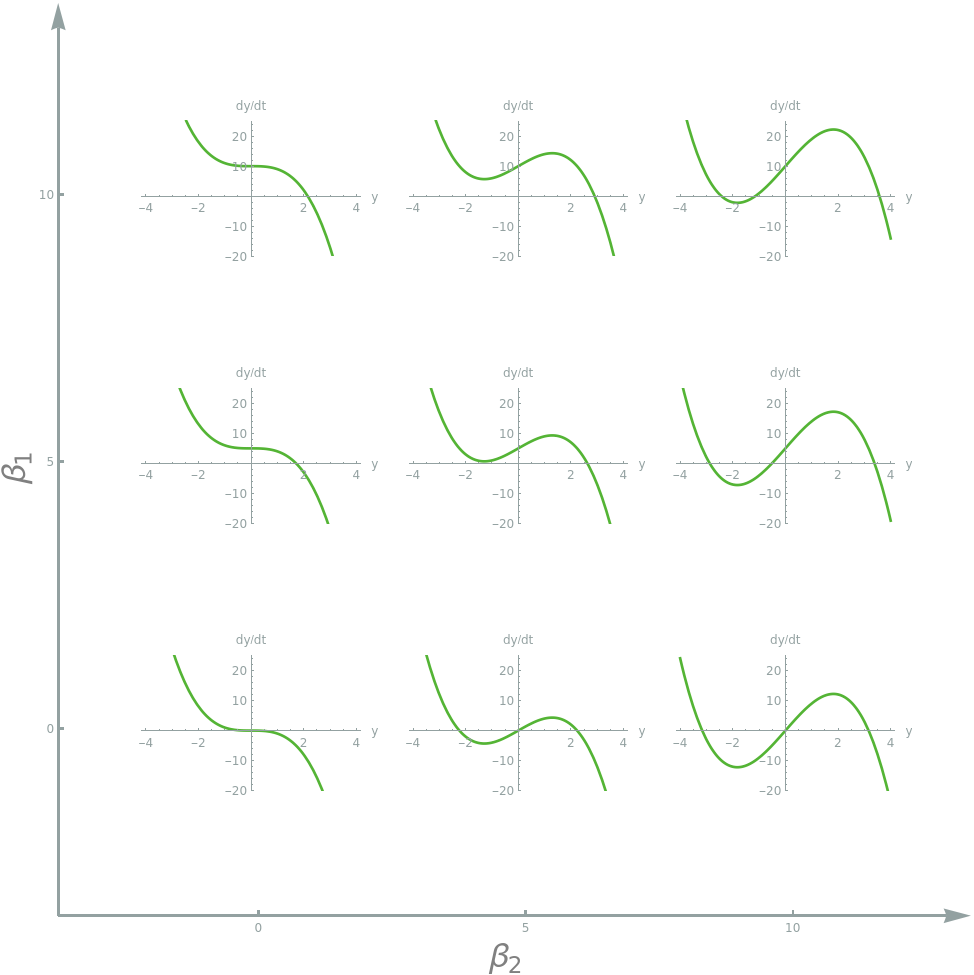
\includegraphics[width=2.1in,angle=0]{./cubic_params.png}
\caption{The effect is that $\beta_2$ determines the curvature around the 
center (horizontal)
and $\beta_1$ determines where the function reaches equilibrium (vertical).
If x-intercept is within the curved region this is an example of bistability.}
\label{cubic_params}
\end{center}
\end{figure}

The aliens are very protective of their young and the experimenters are not able
to observe the process of many aliens coloring to maturity. However,
it is possible for an experimenter to join a cluster of adults and count
how many of each color there are. This is a common case in many experimental 
situations since it is often
easier to sample developmental outcomes than it is to sample longitudinal developmental
trajectories. Luckily our dynamical model gives us an intuitive way of thinking about
what those counts mean. 

If we imagine each individual as a specific trajectory through
the state space of the model then we are simply sampling initial conditions 
and counting how many end up in each basin of attraction, we visualize this 
in Figure \ref{basins}. Each
colored point represents an individual and the color represents their color after
the developmental process. As previously noted the unstable equillibrium acts as a
divider between the two stable equillibrium states. 
Points to
the left will be cyan and points to the right will be magenta. 

\begin{figure}[t]
\begin{center}
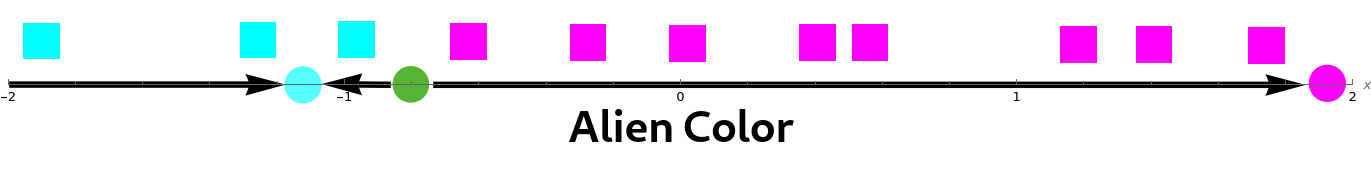
\includegraphics[width=2.1in,angle=0]{./basins.png}
\caption{Here we see the phase portrait of the system. The blue points represent
the stable equillibria and the red point is the saddle node. The magenta volume
represents the region of points that will end up in one basin and the cyan volume
represents the rest of the volume which will end up in the other basin of attraction.
The points above the volumes represent sampled trajectories colored by the 
basin they will end up in.}
\label{basins}
\end{center}
\end{figure}

An unstable attractor is a critical point of the vector field ($\dot{y} = 0$) and
whose derivative is positive ($\ddot{y} > 0$) (cite). 
Based on this criterion we will define a function $f$ which 
takes as inputs two parameters $\beta_1$ and $\beta_2$ and returns the position
of the unstable equilibrium, $SP$.

\begin{eqnarray}
SP = \frac{\sqrt[3]{-6} 
\left(\sqrt{81 \beta_1^2-12 \beta_2^3}-9 \beta_1\right)^{2/3}-2 
(-3)^{2/3} \beta_2}{3\ 2^{2/3} \sqrt[3]
{\sqrt{81 \beta_1^2-12 \beta_2^3}-9 \beta_1}}\\
f(\beta_1,\beta_2) = SP
\end{eqnarray}

\begin{figure}[t]
\begin{center}
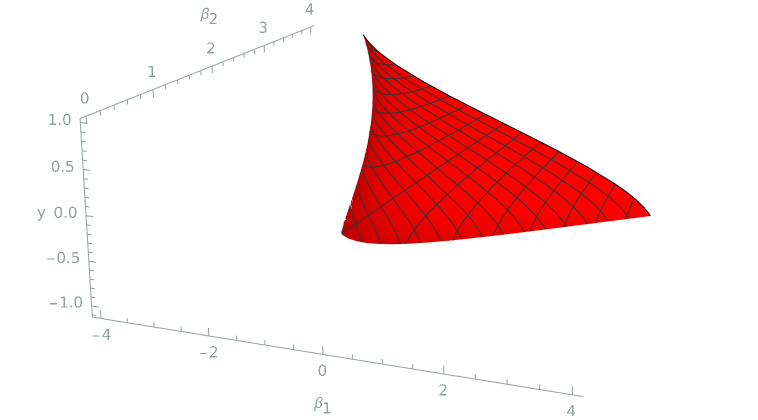
\includegraphics[width=2.1in,angle=0]{./saddle_cubic.png}
\caption{This is the surface of the saddle point location as a function of
the parameter $\beta_1$ and $\beta_2$. The manifold is embedded into probability
dimension representing the probability of a trajectory leading to the cyan attractor.}
\label{cubic_saddle}
\end{center}
\end{figure}

Depending only on $\beta_1$ and $\beta_2$ we
can determine where the saddle point and thus the basins of attractions will be.
Although a little hairy, we were able to derive this function analytically. In 
the more general case identifying the saddle point as a function of parameters 
may require numerical methods. The function itself is visualized in
Figure \ref{cubic_saddle}. 

The alienologists find a fascinating result that there
are always 3 cyan aliens for each 7 magenta aliens. This can be stated as 

\begin{eqnarray}
  P_{cyan} = 0.3\\
  P_{magenta} = 0.7
\end{eqnarray}

This seems to be the case regardless
of which cluster they observe. This is odd because many alienologists have
also observed that $\beta_1$ and $\beta_2$ can vary in different clusters. 
If we consider this puzzle in the context of our dynamical
model, one way to interpret is that we observe a fixed ratio of the basins of
attraction. Intuitively this shouldn't be the case since the different
clusters have different parameters which would imply different basin boundaries.
Although seemingly contrived, as will be detailed later, 
this situation seems to occur in the two
real developmental systems we will discuss in the next sections.

The method we propose assumes that both the interpretation of the model and the
experimental observations are correct. Given these conditions we demonstrate 
how we can make experimental predictions about the relationship between the 
parameters $\beta_1$ and $\beta_2$.

First we must make some assumptions
about how the experiment is conducted. This is the previously mentioned 
sampling distrbution.
This may be known in an emprically studied system but for theoretical 
clarity we will use the maximum entropy uniform distribution. We will also add
bounds to this distribution so as to meet the integral requirment for 
probabilities. For this example we take $y_{min} = -2$ and $y_{max} = 2$.
Thus equation \ref{bound_uniform} becomes:
\begin{eqnarray}
  \label{p_cubic}
    P(y) = \begin{cases}
        \frac{1}{2 - (-2)} & \text{ for } -2\leq y\leq 2\\
        0 & \text{otherwise}
    \end{cases}
\end{eqnarray}

We now have $f(\beta_1,\beta_2), P(y)$, and $P_{cyan}$. These are all the 
ingredients necessary to identify the relation 
\[h(\beta_1) = \beta_2\]

Plugging in the known constant into equation (4), we get:
\begin{eqnarray}
  P_{cyan} = 0.3 = \int_{-\infty}^{SP} P(y)dy
\end{eqnarray}

The next step is to solve for $SP$. In this case, because of our choice $P(y)$
we can solve for $SP$ analytically. Since $P_{cyan}$ is neither 1 nor 0 we know 
that $SP \in [y_{min},y_{max}]$:

\begin{eqnarray}
  SP = P_{cyan}(y_{max}-y_{min}) + y_{min} = -0.8
\end{eqnarray}

\begin{figure}[t]
\begin{center}
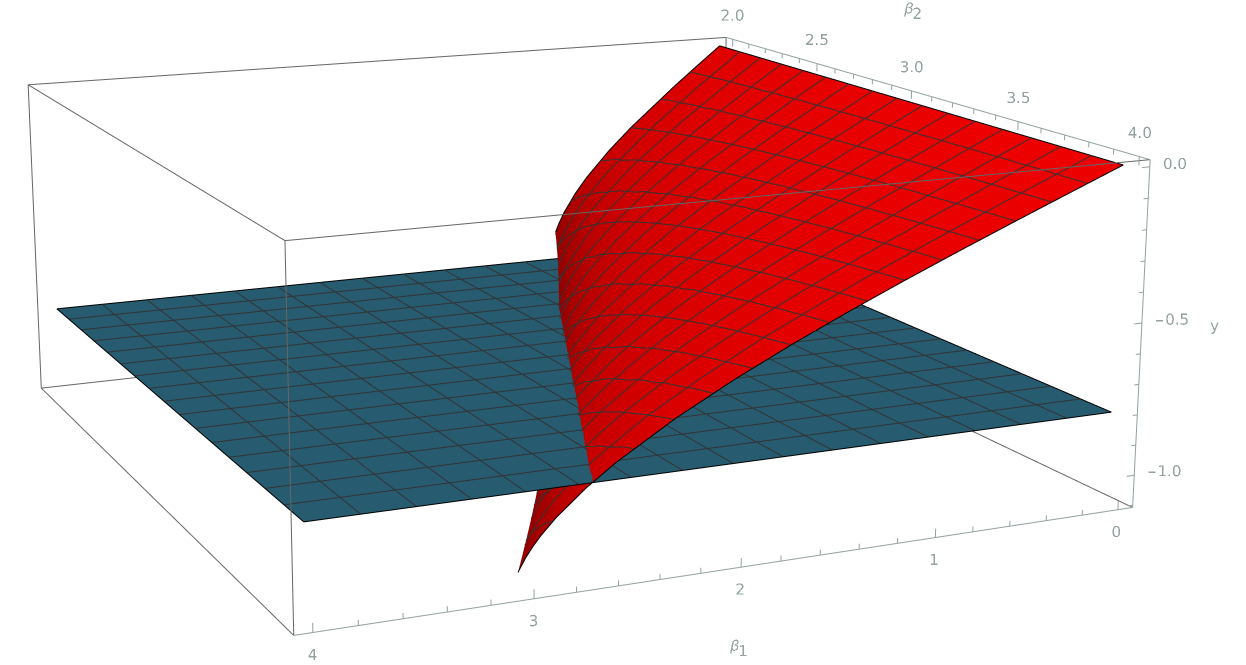
\includegraphics[width=2.1in,angle=0]{./cubic_h.png}
\caption{This is the surface of the saddle point location as a function of
the parameter $\beta_1$ and $\beta_2$, intersected with a plane at $SP=-0.8$.
The intersection represents the parameter relation $h$.}
\label{cubic_h}
\end{center}
\end{figure}

The last step in this process is to invert the function $f(\beta_1,\beta_2)$ 
and use the found value of $SP$ to identify a relation $h$ on $\beta_1$ and $\beta_2$.
One way to visually intepret this relation is presented in Figure \ref{cubic_h}.
The fixed probability acts as a plane that intersects the y-axis exactly at the
saddle point. Thus the model parameters are no longer just defined by the whole
saddle manifold but instead are restricted to points along that manifold that intersect
with this plane. 


\begin{eqnarray}
    \beta_1 = h(\beta_2) = -0.512 + 0.8 \beta_2
\end{eqnarray}

Once again the simplicity of our example makes it possible to analytically 
solve this problem
by taking the inverse of $f$ and solving for $f(\beta_1,\beta_2) = -0.8$.
In general however, we might need to make a numerical
approximation to be able to determine this relation. This will come up in the 
later examples.

The line $h$ is a fixed relationship between
the two parameters, $\beta_1$ and $\beta_2$ that must be satisfied for us to 
unify the experimental observation with
our model. Hence we expect that if the experimenters were to measure $\beta_1$ and 
$\beta_2$ they would fall on the line satisfying the equation. An alienologist 
should then be able to predict $\beta_1$ or $\beta_2$ given that they
know the other. This relation thus gives us a whole new way to validate or
falsify our original model. 

Now that we have established the steps to apply the method in a simple case we will now 
consider the same sequence of operations in the case of two models of real world experimental
systems. Although we may need to use numerical approximations and our parameters may not
be easily interpretable we will see that the same steps can be applied.

\subsection{Infant Prehension}

Infant prehension or reach-to-grasp is an important developmental milestones 
for many primates including humans (cite). Not only is the behavior itself
functionally important (cite) but also serves as a foundation for more general motor
coordination skills (cite) and many social skills (cite). The development of 
reach-to-grasp
has therefore been an important model system in the study of human development (cite). 
One way of modeling prehension development has been to look at a phase transition
between reach and reach-to-grasp. Infants begin to reach before they preform grasps and
one set of hypothesese has interpreted this as a phase transition into bistability (cite). 
Experimental work in this direction has been complemented by modeling of this phase
transition. This makes prehension a potential model system for exploring developmental
dynamics with the tools of dynamical systems theory.

Much like our alien example, experiments in prehension development 
have shown that after
the emergence of grasping we observe a narrow probability distribution 
while bistability
remains. Although infants eventually will grasp with every reach until 
then, there seems to
be a fixed probability distribution of reaching-to-grasp and 
reaching-without-grasp (cite).
We will treat this as meaning there is a constant probability across 
both stable outcomes,
however, extensions of this work could improve the method to account for
more complex distributions.
Either way the fact that the probability distribution is narrow is still 
enough to suggest
there may be an important relation between the model parameters.

There is a major difference between this example and our previous example however. 
In the previous  section we demonstrated how this method can be applied to a simple
toy model and how given an experimentally observed probability we could make a prediction
about the model parameters. In many cases the exact model parameters are 
not singular observables but instead are a function of observables. In such cases we 
must accommodate the method by relating the saddle point position not to the model
parameters but to the desired experimental observable. 
This will be the case as we apply the method to a model of the development of 
reach-to-grasp in infants. 

We consider the dynamical model of prehension development proposed by 
Wimmers et al. (cite). This
model considers two stable states: reach-to-grasp and reach-without-grasp. 
To develop this
model the researchers looked at many possible parameters and considered 
their effect on 
the resulting probability of either of the bistable outcomes. 
They found that the results
were best explained a by version of the cubic equation.

\begin{eqnarray}
  \dot{y} = \beta_1 + \beta_2 (\frac{x-51.04}{26.98}) - (\frac{x-51.04}{26.98})^3
\end{eqnarray}
where
\begin{eqnarray}
  \beta_1 = 5.98 - 1.07c + 31.92w\\
  \beta_2 = 5.56 - 0.25c + 0.38w
\end{eqnarray}

Notice that this equation is quite similar to the cubic however both $\beta_1$ and 
$\beta_2$ are linear sums of other parameters: $c,w$ 
where $c$ is the arm circumference
of the infant and $w$ is the arm weight. 
The value of $x$ is shifted linearly this does 
not affect the actual dynamics and is ignored for methodological clarity. 
We are no longer
interested in how the values of $\beta_1$ and $\beta_2$ relate to $SP$. 
Instead we will
consider how $SP$ is related to $c,w$. 
However, almost all of the other steps will be the
same as in the previous example.

First we visualize the contributions of the paramaters to the dynamics 
(Figure \ref{fig5}).
Since the paramaters affect both $\beta_1$ and $\beta_2$ we cannot simply attribute 
curvature to one and x-intercept location to the other. 
Instead we see that both parameters
affect both of these properties however the contribution of 
$w$ to the x-intercept location
is significantly greater than the contribution of $c$. 
This will play a role in how the
manifold looks once it is embedded in the state space 
(Figure \ref{prehension_saddle}).

\begin{figure}[t]
\begin{center}
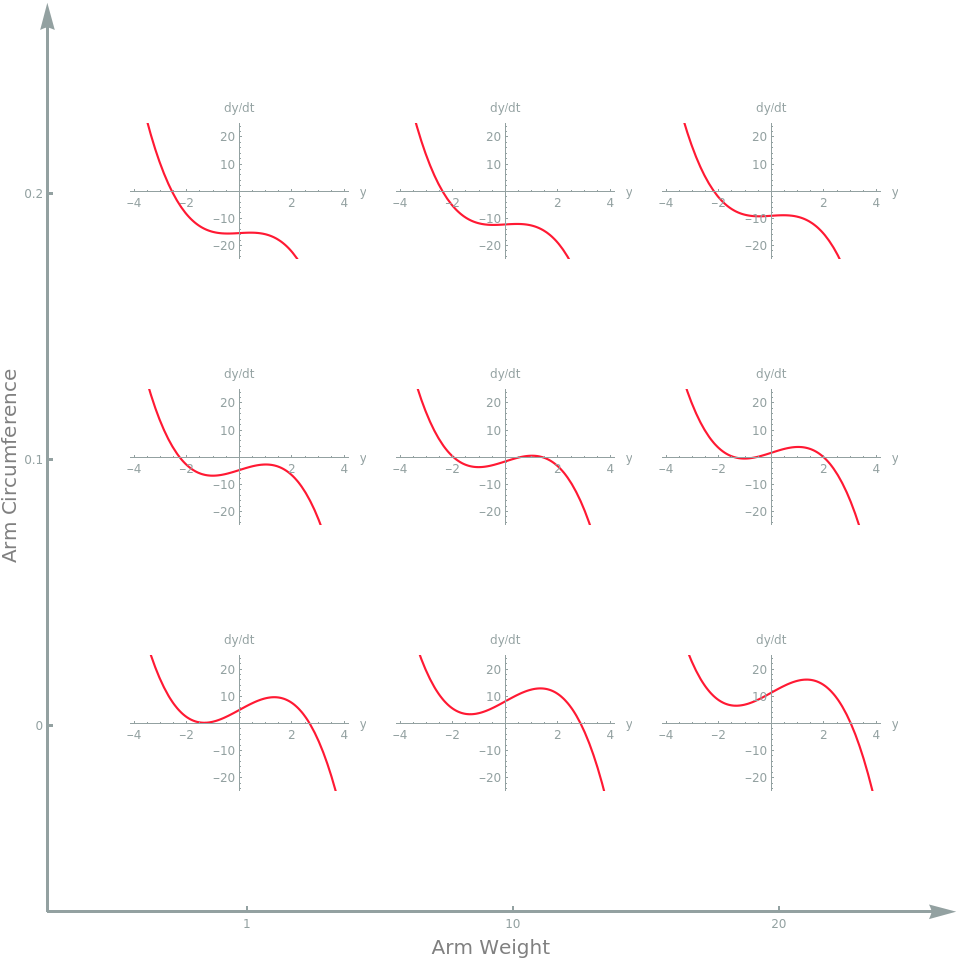
\includegraphics[width=2.1in,angle=0]{./prehension_params.png}
\caption{3x3 grid of variation in $c$(horizontal) $w$(vertical). Unlike the previous
model curvature and x-intercept position changes as a function of both parameters.}
\label{fig5}
\end{center}
\end{figure}

Once again we need to start by defining the relationship between $SP$ and 
the parameters.
This will again take the form of a function $f(c,w)$ that returns the 
saddlepoint location 
$SP$.
Luckily since $\beta_1$ and $\beta_2$ are only linear combinations of $c,w$ we can still
find the function $f(c,w)$ analytically. Although the closed form 
has been omitted due to length
complexity. It is visualized in Figure \ref{prehension_saddle}.

\begin{eqnarray}
  SP = f(c,w)
\end{eqnarray}

As before we again
need to define a sampling distrubition. We will do this using a bounded uniform
pdf for $P(y)$ which is identical to $P(y)$ in equations (3, 13). 
The only difference being the bounds in this case
\[
  y_{min} = 0
  \] 
  and 
  \[y_{max} = 100\]

This the volumes represent whether the behavior of grasping
is preformed rather than the alien's mature
color. Using the same reasoning we can define the desired $P_{grasp}(y)$, 
the probability
that in a sampled point the baby will grasp, by integrating the volume. In this case
the desired volume is on the right of the unstable equillibrium 
so we integrate from $SP$ to $\infty$.

\begin{eqnarray}
    P_{grasp}(y) = \int_{SP}^{\infty}P(y)dy
\end{eqnarray}

\begin{figure}[t]
\begin{center}
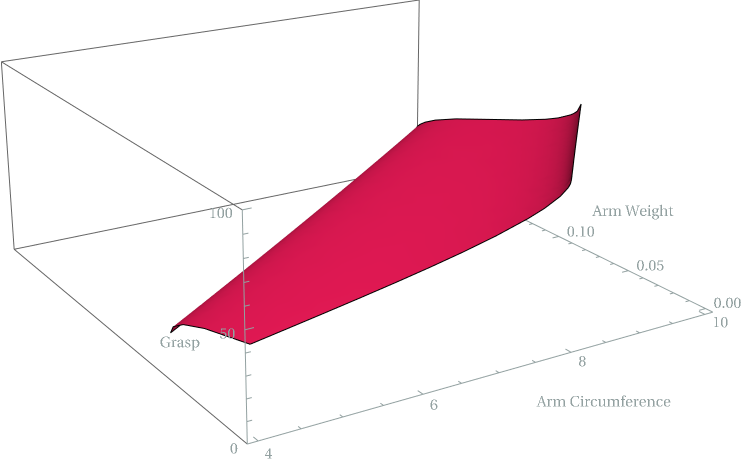
\includegraphics[width=2.1in,angle=0]{./saddle_prehension.png}
\caption{The probability we find as we vary saddlepoint by moving in the 
parameter space of $c,w$. The plane represents the observed constant probability 
distribution.}
\label{prehension_saddle}
\end{center}
\end{figure}

As before any pair $c,w$ will define an $SP$ and thus a $P_{grasp}$. Unlike 
our hypothetical the real world is not nearly as neat. Experimental evidence suggests
a distrbution of $P_{grasp}$ rather than a singular constant. However, for this paper
we will simply pick the mean of this distrbution and treat it as a constant although,
future work could extend the method to a distrbution of probabilites instead.

\begin{eqnarray}
  P_{grasp} = 0.5
\end{eqnarray}

Once again we use the integral to solve for $SP$ in relation to the probabilty. This
will give us a value for $SP$ which we can then use for restricting our parameters.

\begin{eqnarray}
  SP = P_{grasp}(y_{max}-y_{min}) + y_{min} = 50
\end{eqnarray}

As before we simply plot this $SP$ as a plane which intersects the saddle manifold
in parameter space as in Figure \ref{prehension_h}. We see once again this intersection
forms a 1D curve through parameter space. However, unlike before we cannot write it 
in closerd form.

\begin{figure}[t]
\begin{center}
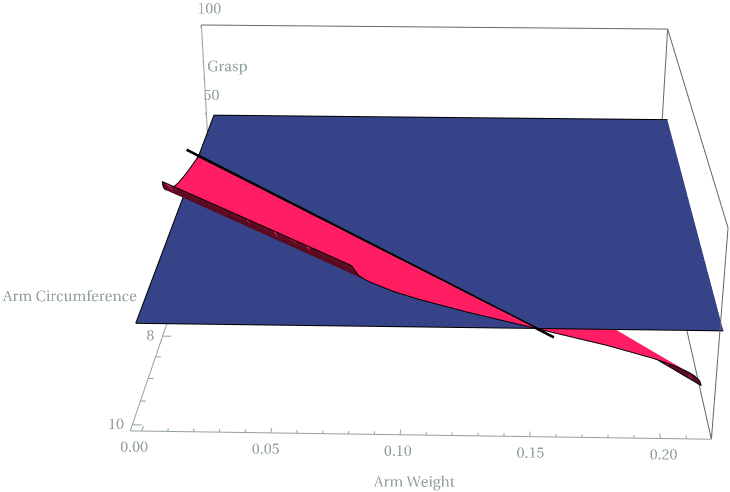
\includegraphics[width=2.1in,angle=0]{./prehension_h.png}
\caption{The probability we find as we vary saddlepoint by moving in the 
parameter space of $c,w$. The plane represents the observed constant probability 
distribution.}
\label{prehension_h}
\end{center}
\end{figure}

This curve, makes a prediction that the fixed probability 
distribution implies a
relation between arm circumference and arm weight. As one parameter varies 
the other should at a proportional degree along the drawn curve.
We now have a prediction that can falsify or 
further validate the cusp model fit in the 
orignal paper (cite).

In this example we applied the same steps and method to a real world system. 
We showed how
more complex parameter relations can be accounted for by adjusting the 
function $f$ and how
different parameterizations might imply more complex relations to the 
resultant probabilites.
However, since our model was still cubic we were able to use much of 
the same analytical 
machinery. We will next consider a case where the model is much more 
complex, yet we will 
show with the use of numerical approximation how many of the same 
steps can be applied.

\subsection{Planerian Regeneration}

The final case we consider is a model of planerian flatworm regeneration. The dynamics 
of this system are much more complicated and many of the analyitcal tools we used
in the previous examples no longer apply. Instead, we will demonstrate how numerical
approximations may be used to fill in the gaps.

Planerian flatworm is a popular model system for several reasons (cite). Of particular
interest to us is it's regenerative capabilities. Work from the Levin lab (cite) has
provided a wide range of experimental results that has helped characterize the development
of this animal across many conditions. For this example we will consider axial patterning
in the flatworm.

Planerian can reproduce through an asexual cloning process. When a worm is cut into two
the head and the tail will both regrow the rest of the body. One interesting aspect of
this process is that it seems to be at least in part controlled by electrical signaling
rather than purely chemical signaling. This has been show through experimental manipulation
of the polarity of the environment during regeneration(cite).

Through manipulation of the polarity of the environment it becomes possible to cause
the planerians decapatated head to grow another head instead of a tail, resulting
in a two headed worm. Interestingly, there is a more surprising finding. It is also
possible to manipulate the polarity such that the worm regrows normally however if 
cut again the worm may grow another head or a tail stochasticlly. Such worms are 
called cryptic worms (cite). One unexpected experimental result is that near universally
cryptic worms have a $25\%$ chance of spawning into a two-headed worm and a 
$75\%$ chance 
of spawing another cryptic worm.

Many features of this phenomena have been successfully modeled using a bistable dynamical
model. Normal and double headed worms are modeled as living in parameter space without
bistability where as cryptic worms are thought to occuppy the bistable region (cite). 
This is the model we will use for the rest of this example.

\begin{eqnarray}
  \dot{y}=-\frac{2 (g_{max}-0.02) y}{1\, +0.0000454 e^{-0.5 y}
  +0.0000454 e^{0.5 y}}+70 g_{pol}-4.09 y-280
\end{eqnarray}

We have simpliefied the model significantly from it's original formulation by replacing
parameters with their experimentally observed values. We have also reduced this from a 
2D to a 1D system by considering the difference in polarity 
between head and tail rather
than head and tail as seperate dimensions. This works in this case 
because the difference
in polarity is sufficient for applying the method.
This leaves us with two free parameters
$g_{pol},g_{max}$. $g_{pol}$ is the intrinsic polarity of the head cells
and $g_{max}$ is the maximum conductance across the gap junction.

Once again we will start by considering how the parameters affect the equillibria of
the model. This is will give us intuitions about how they may affect the probability
surface. We can visualize this in Figure \ref{fig7}. Although no longer cubic we 
see a similar pattern as before where one parameter mainly affects the curvature 
($g_{max}$)
and one mainly affects the x-intercept location ($g_{pol}$). 
Although these parameters are 
definitely not linearly decomposable as before.

\begin{figure}[t]
\begin{center}
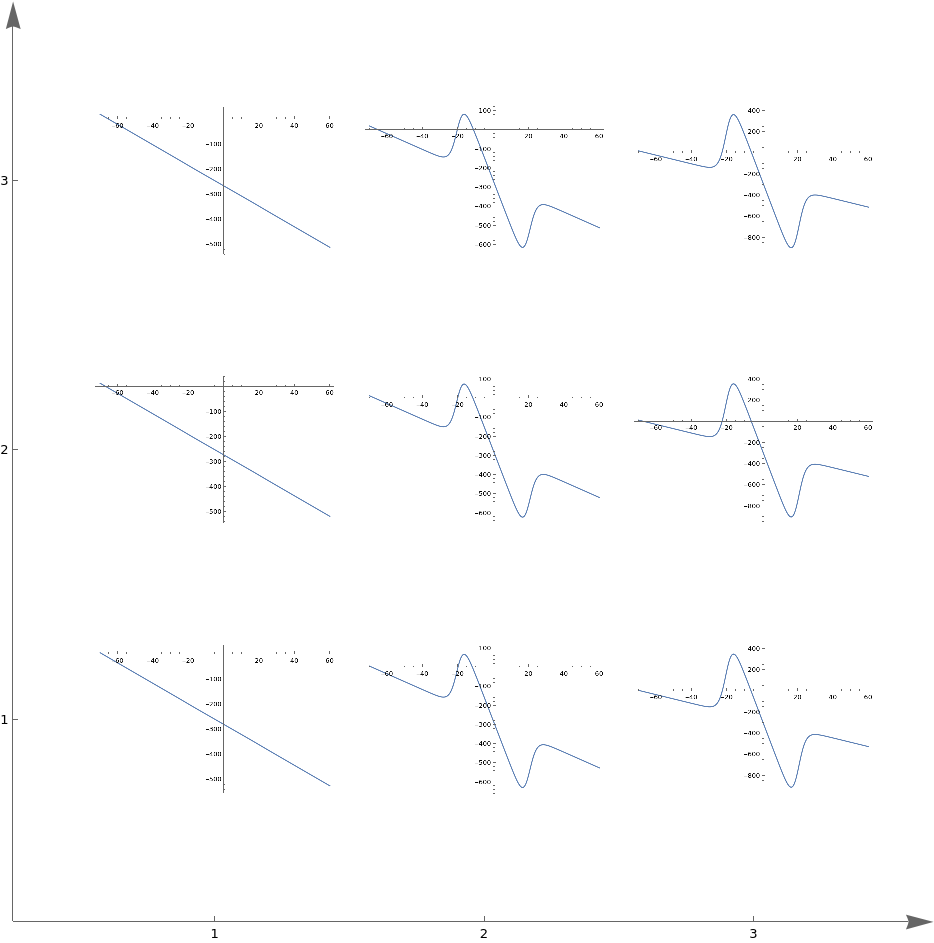
\includegraphics[width=2.1in,angle=0]{./worm_params.png}
\caption{Vector field function as we vary the two parameters}
\label{fig7}
\end{center}
\end{figure}

Again we go through the process of defining a function $f(g_{pol},g_{max})$ that
given the two parameters of the model will return the equillibria location. Unlike 
before we cannot simply solve for the conditions relevant to a saddlepoint. Instead
we must resort to numerical root finding. We identify an initial guess for the 
saddlepoint 
by looking at Figure \ref{fig7}. The middle intersection on the x-axis is the 
saddlepoint.
Using this guess we can generate a tensor whose first 2 dimensions are the parameters 
$g_{pol}$ and $g_{max}$ and whose 3rd dimension is the saddlepoint location. This also
defines a surface which we can plot (Figure \ref{worm_sp}).

\begin{figure}[t]
\begin{center}
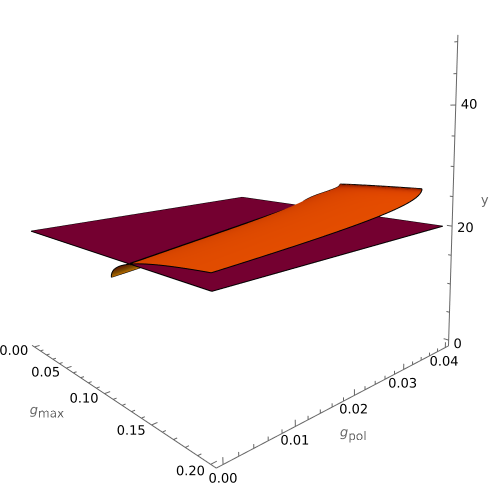
\includegraphics[width=2.1in,angle=0]{./worm_saddle.png}
\caption{Saddle point location as a function of the two parameters: 
$g_{pol}$ and $g_{max}$.}
\label{worm_sp}
\end{center}
\end{figure}

This system is another example of the relatively constant state distrbution phenomenon.
Here the two possible attractors are $P_{cryptic}$ and $P_{two-headed}$. Once again,
we take the liberty of assuming these distributions are constant rather than simply 
narrow. Informed by experimental data (cite)

\begin{eqnarray}
  P_{cryptic} = 0.75
\end{eqnarray}

Using the same methodology as before we derive the value od $SP$ this time we bound
our sampling space with $[-80,0]$ which is roughly the range of cellular polarity. 
Using this and the integral from equation (4):

\begin{eqnarray}
  SP = P_{cryptic}(y_{max}-y_{min}) + y_{min} = -20
\end{eqnarray}

This is the plane that we observe in Figure \ref{worm_prob}. The intersection
of the plane and the manifold is our predicted parameter range. In this to derive
this figure we had to apply numerical calculations since $f(c,w)$ could not be 
expressed in closed form

\begin{figure}[t]
\begin{center}
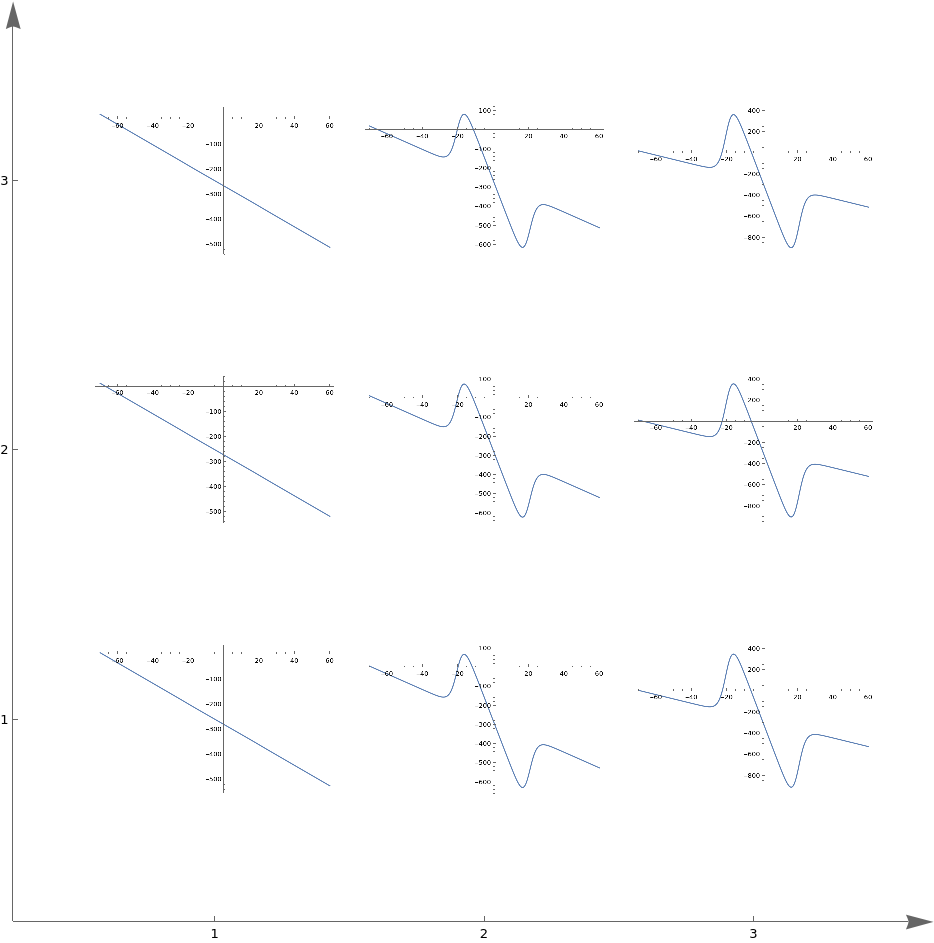
\includegraphics[width=2.1in,angle=0]{./worm_params.png}
\caption{Worm parameter manifold embedded in probability space}.
\label{worm_prob}
\end{center}
\end{figure}

Once again we can see how the constant probability distribution presents a set of 
constraints on the parameters of the dynamical model. In turn such constraints can
be used to make emprical predictions which can further validate or contradict the
model as a hypothesis. Thus we can make concrete predictions on what the parameters
should be even in the case of an extremely simplified theoretical model.

\section{Discussion}
In this paper we have demonstrated how our method can be applied to different
dynamical models to make concrete predictions about observable paramaters using 
a theoretical model in conjunction with experimental data. We also demonstrate
how this model can be applied to real world systems even when things become 
analytically intractable.

Although in this work we limited our model to a very simple sampling distribution,
using the known emprical sampling distrbution could greatly improve the accuracy of
the method without comprimising the conceptual steps, albeit with increased numerical
computationa time.

Future work may extend this method in many different directions. One example may 
be to introduce more complex parameter constraints than a constant probability
distribution. Having a range of possible probabilities will also reduce the
range of possible parameters for the models. Even more generally an observable
of the equillibria could be used with a similar method rather than simply
probabilities. As long as the function can be related to the equillibria of the
dynamics it can serve as a means of inferring necessary dynamical parameter relations.

Finally, we demonstrate that dynamical systems can not only serve as a set of conceptual
tools but also can help elucidate and imporove experimental results. There is much need
for growing communication between experiment and theory in biology and dynamical systems
can provide a firm foundation for such communication.
\section{Acknowledgements}

This work was supported by NSF grant No.\ PHY-9723972.

\footnotesize
\bibliographystyle{apalike}
\bibliography{example} % replace by the name of your .bib file


\end{document}
